\documentclass{article}

\usepackage[margin=0.5in,bottom=1in,footnotesep=1in]{geometry}

\usepackage{amsmath}


\usepackage{multicol}
\setlength{\columnsep}{1cm}
\usepackage[]{algorithm2e}

\usepackage{lipsum}% for dummy text
\usepackage[varg]{txfonts}
\usepackage{graphicx}
\usepackage{subcaption}
\usepackage{multirow}

\usepackage[font=small,labelfont={sf,bf}]{caption}


\usepackage{titlesec}
\titleformat{\section}{\fontfamily{phv}\fontsize{12}{15}\bfseries}{\thesection}{1em}{}
\titleformat{\subsection}{\fontfamily{phv}\fontsize{10}{15}\itshape}{\thesubsection}{1em}{}

\title{\textbf{FYS4150 Project 3: \\Numerical integration}}
\author{Marie Foss, Maria Hammerstr{{\o}}m}
\date{} % removes date from title

\begin{document}

\maketitle

\begin{abstract}
	\noindent \lipsum[1]
	\vspace*{2ex}
	
	\noindent \textbf{Github:} \textit{https://github.com/mariahammerstrom/Project3}
	\vspace*{2ex}
\end{abstract}



\begin{multicols}{2}

\section{Introduction}
In this project we will determine the ground state correlation energy between two electrons in an helium atom by calculating a six-dimensional integral that appears in many quantum mechanical applications. The methods we will use are Gauss-Legendre and Gauss-Laguerre quadrature and Monte-Carlo integration. 

We assume that the wave function of each electron can be modeled like the single-particle wave function of an electron in the hydrogen atom. The single-particle wave function  for an electron $i$ in the $1s$ state  is given in terms of a dimensionless variable    (the wave function is not properly normalized)

\begin{equation*}
	{\bf r}_i =  x_i {\bf e}_x + y_i {\bf e}_y +z_i {\bf e}_z ,
\end{equation*}
as

\begin{equation*}
	\psi_{1s}({\bf r}_i)  =   e^{-\alpha r_i},
\end{equation*}
where $\alpha$ is a parameter and 

\begin{equation*}
	r_i = \sqrt{x_i^2+y_i^2+z_i^2}.
\end{equation*}
We will fix $\alpha=2$, which should correspond to the charge of the helium atom $Z=2$. 

The ansatz for the wave function for two electrons is then given by the product of two 
so-called $1s$ wave functions as 

\begin{equation}
	\Psi({\bf r}_1,{\bf r}_2)  =   e^{-\alpha (r_1+r_2)}.
\end{equation}
The integral we need to solve is the quantum mechanical expectation value of the correlation energy between two electrons which repel each other via the classical Coulomb interaction, namely

\begin{equation}\label{eq:correlationenergy}
	\langle \frac{1}{|{\bf r}_1-{\bf r}_2|} \rangle = \int_{-\infty}^{\infty} d{\bf r}_1d{\bf r}_2  e^{-2\alpha (r_1+r_2)}\frac{1}{|{\bf r}_1-{\bf r}_2|}.
\end{equation}
This integral can be solved in closed form, which gives an answer of $5\pi^2/16^2 \approx 0.192765710958777$.



\section{Methods}

\subsection{Gauss-Legendre and Gauss-Laguerre quadrature}
Gaussian quadrature (hereafter GQ) is a method that solves integrals with excellent results, giving high precision for few integration points, compared to simpler integration methods such as Newton-Cotes quadrature. 

The basic idea behind all integration methods is to approximate the integral

\begin{equation}
	I = \int_a^b f(x) dx \approx \sum_{i = 1}^N \omega_i f(x),
\end{equation}
where $\omega$ are the weights and $x$ are the chosen mesh points. The theory behind GQ is to obtain an arbitrary weight $\omega$, which will not be equally spaced, through the use of orthogonal polynomials, namely Legende and Laguerre polynomials in this case. For GQ we thus make the approximation

\begin{equation}
	f(x) \approx P_{2N-1} (x),
\end{equation}
where $P_{2N-1} (x)$ is a polynomial of degree $2N-1$ with N mesh points. The mesh points are the zeros of the chosen orthogonal polynomial of order $N$, and the weights are determined from the inverse of a matrix defined by the orthogonal polynomials. Thus, GQ says that

\begin{equation}
	\int f(x) dx \approx \int P_{2N-1}(x) dx \approx \sum_{i = 1}^{N-1} P_{2N-1}(x_i) \omega_i.
\end{equation}
The \textbf{Legendre polynomials} are solutions to a differential equation arising in for example the solution of the \textit{angular dependence} of Schr\"{o}dinger's equation with spherically symmetric potentials such as the Coulomb potential. The Legendre polynomials are defined as

\begin{equation}
	L_k(x) = \frac{1}{2^k k!} \frac{d^k}{dx^k} (x^2 - 1)^k \textrm{ , } k = 0,1,2, \dots
\end{equation}
Using \textbf{Gauss-Legendre quadrature} means solving an integral from $- \infty$ to $+ \infty$. This can however not be achieved numerically. To find out how we can substitute the infinite limits with finite limits, we plot the single-particle wave function shown in Fig.~\ref{fig:integrand}, which shows that the function $e^{-\alpha r_i}$ reaches zero at approximately $r_i \approx 3$. We therefore used the limits [-3,3].

\begin{center}
	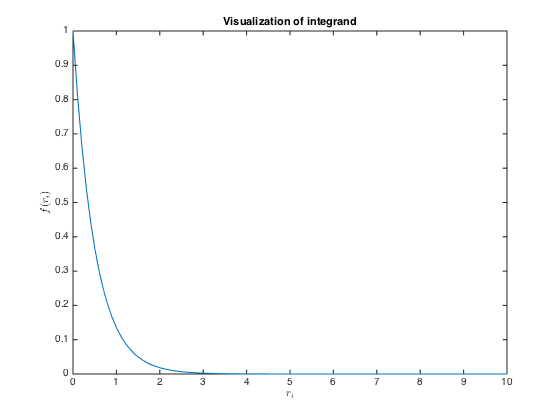
\includegraphics[width=90mm]{integrand.png} 	
	\captionof{figure}{The single-particle wave function $e^{-\alpha r_i}$.}
	\label{fig:integrand}
\end{center}


Similarly, the \textbf{Laguerre polynomials} are solutions to the differential equation arising in for example the solution of the \textit{radial} Schr\"{o}dinger's equation as described above. The Laguerre polynomials are defined as

\begin{equation}
	L_n(x) = e^x \frac{d^n}{dx^n} (x^n e^{-x}) \textrm{ , } n = 0,1,2, \dots
\end{equation}
When using Gauss-Laguerre quadrature the integral runs from zero to $\infty$. The integral can be rewritten with spherical coordinates to better deal with the infinite limits. Then the integral in Eq. (\ref{eq:correlationenergy}) becomes:

\begin{equation}
	I = \int_0^{2\pi} \int_0^{2\pi}  \int_{-1}^1 \int_{-1}^1   \int_0^{\infty} \int_0^{\infty}    \frac{r_1^2 r_2^2}{r_{12}} dr_1  dr_2 dcos(\theta_1)dcos(\theta_2)d\phi_1d\phi_2
\end{equation}
with

\begin{equation*}
\frac{1}{r_{12}}= \frac{1}{\sqrt{r_1^2+r_2^2-2r_1r_2cos(\beta)}},
\end{equation*}
where

\begin{equation*}
cos(\beta) = cos(\theta_1)cos(\theta_2)+sin(\theta_1)sin(\theta_2)cos(\phi_1-\phi_2)).
\end{equation*}



\subsection{Monte Carlo}
The Monte Carlo method is a statistical simulation method which can be used for systems that are described by their probability distribution functions (PDFs). The Monte Carlo method proceeds by random samplings from the PDF. The final result is taken as an average over the number of simulations.

We also want to run the Monte Carlo method by using importance sampling. In the regular Monte Carlo method we use uniformly distributed random numbers, but when considering importance sampling we will instead use exponentially distributed random numbers. We will also switch to spherical coordinates.
... 


\section{Results}
The \textbf{time} taken to run the program was recorded for the various methods:

\begin{center}
\begin{tabular}{ l l l l l}\hline
	Method 				& N	 		&I			&$\sigma$		& $t$ (s) \\ \hline
	Gauss-Legendre 		& 25 			& 0.1958		& -				& 6 \\
	Gauss-Laguerre 		& -			& -			& -				& - \\
	Monte Carlo 			& 500E5 		& 0.1972		& -3.88679E-2		& 6 \\
	Monte Carlo * 			& 1E5		& 0.1959		& -3.61967E-2		& 0 \\
	\hline
\end{tabular}
\end{center}
where * denotes importance sampling.

COMMENTS.



\section{Conclusions}
...





\section{List of codes}

The codes developed for this project are:\\
...

\end{multicols}

\end{document}
